\documentclass[twoside]{book}

% Packages required by doxygen
\usepackage{calc}
\usepackage{doxygen}
\usepackage{graphicx}
\usepackage[utf8]{inputenc}
\usepackage{makeidx}
\usepackage{multicol}
\usepackage{multirow}
\usepackage{textcomp}
\usepackage[table]{xcolor}

% NLS support packages
\usepackage[spanish]{babel}
% Font selection
\usepackage[T1]{fontenc}
\usepackage{mathptmx}
\usepackage[scaled=.90]{helvet}
\usepackage{courier}
\usepackage{amssymb}
\usepackage{sectsty}
\renewcommand{\familydefault}{\sfdefault}
\allsectionsfont{%
  \fontseries{bc}\selectfont%
  \color{darkgray}%
}
\renewcommand{\DoxyLabelFont}{%
  \fontseries{bc}\selectfont%
  \color{darkgray}%
}

% Page & text layout
\usepackage{geometry}
\geometry{%
  a4paper,%
  top=2.5cm,%
  bottom=2.5cm,%
  left=2.5cm,%
  right=2.5cm%
}
\tolerance=750
\hfuzz=15pt
\hbadness=750
\setlength{\emergencystretch}{15pt}
\setlength{\parindent}{0cm}
\setlength{\parskip}{0.2cm}
\makeatletter
\renewcommand{\paragraph}{%
  \@startsection{paragraph}{4}{0ex}{-1.0ex}{1.0ex}{%
    \normalfont\normalsize\bfseries\SS@parafont%
  }%
}
\renewcommand{\subparagraph}{%
  \@startsection{subparagraph}{5}{0ex}{-1.0ex}{1.0ex}{%
    \normalfont\normalsize\bfseries\SS@subparafont%
  }%
}
\makeatother

% Headers & footers
\usepackage{fancyhdr}
\pagestyle{fancyplain}
\fancyhead[LE]{\fancyplain{}{\bfseries\thepage}}
\fancyhead[CE]{\fancyplain{}{}}
\fancyhead[RE]{\fancyplain{}{\bfseries\leftmark}}
\fancyhead[LO]{\fancyplain{}{\bfseries\rightmark}}
\fancyhead[CO]{\fancyplain{}{}}
\fancyhead[RO]{\fancyplain{}{\bfseries\thepage}}
\fancyfoot[LE]{\fancyplain{}{}}
\fancyfoot[CE]{\fancyplain{}{}}
\fancyfoot[RE]{\fancyplain{}{\bfseries\scriptsize Generado el Lunes, 8 de Julio de 2013 00:36:53 para Sudoku por Doxygen }}
\fancyfoot[LO]{\fancyplain{}{\bfseries\scriptsize Generado el Lunes, 8 de Julio de 2013 00:36:53 para Sudoku por Doxygen }}
\fancyfoot[CO]{\fancyplain{}{}}
\fancyfoot[RO]{\fancyplain{}{}}
\renewcommand{\footrulewidth}{0.4pt}
\renewcommand{\chaptermark}[1]{%
  \markboth{#1}{}%
}
\renewcommand{\sectionmark}[1]{%
  \markright{\thesection\ #1}%
}

% Indices & bibliography
\usepackage{natbib}
\usepackage[titles]{tocloft}
\setcounter{tocdepth}{3}
\setcounter{secnumdepth}{5}
\makeindex

% Hyperlinks (required, but should be loaded last)
\usepackage{ifpdf}
\ifpdf
  \usepackage[pdftex,pagebackref=true]{hyperref}
\else
  \usepackage[ps2pdf,pagebackref=true]{hyperref}
\fi
\hypersetup{%
  colorlinks=true,%
  linkcolor=blue,%
  citecolor=blue,%
  unicode%
}

% Custom commands
\newcommand{\clearemptydoublepage}{%
  \newpage{\pagestyle{empty}\cleardoublepage}%
}


%===== C O N T E N T S =====

\begin{document}

% Titlepage & ToC
\hypersetup{pageanchor=false}
\pagenumbering{roman}
\begin{titlepage}
\vspace*{7cm}
\begin{center}%
{\Large Sudoku }\\
\vspace*{1cm}
{\large Generado por Doxygen 1.8.4}\\
\vspace*{0.5cm}
{\small Lunes, 8 de Julio de 2013 00:36:53}\\
\end{center}
\end{titlepage}
\clearemptydoublepage
\tableofcontents
\clearemptydoublepage
\pagenumbering{arabic}
\hypersetup{pageanchor=true}

%--- Begin generated contents ---
\chapter{Clase Q\-Tablero \textbackslash{}n Lenguajes de programación}
\label{index}\hypertarget{index}{}\par
 Profesor\-: Javier Tibau \par
 

 \begin{DoxyAuthor}{Autor}
Marlon Loayza 

Adrián Aguilar 
\end{DoxyAuthor}
\begin{DoxyDate}{Fecha}
08 de Julio del 2013 
\end{DoxyDate}

\chapter{Indice jerárquico}
\section{Jerarquía de la clase}
Esta lista de herencias esta ordenada aproximadamente por orden alfabético\-:\begin{DoxyCompactList}
\item \contentsline{section}{hilo}{\pageref{classhilo}}{}
\item Q\-Dialog\begin{DoxyCompactList}
\item \contentsline{section}{nivel}{\pageref{classnivel}}{}
\item \contentsline{section}{principal}{\pageref{classprincipal}}{}
\end{DoxyCompactList}
\item Q\-Main\-Window\begin{DoxyCompactList}
\item \contentsline{section}{Q\-Tablero}{\pageref{class_q_tablero}}{}
\end{DoxyCompactList}
\item Q\-Widget\begin{DoxyCompactList}
\item \contentsline{section}{hilo1}{\pageref{classhilo1}}{}
\end{DoxyCompactList}
\end{DoxyCompactList}

\chapter{Índice de clases}
\section{Lista de clases}
Lista de las clases, estructuras, uniones e interfaces con una breve descripción\-:\begin{DoxyCompactList}
\item\contentsline{section}{\hyperlink{classhilo}{hilo} }{\pageref{classhilo}}{}
\item\contentsline{section}{\hyperlink{classhilo1}{hilo1} }{\pageref{classhilo1}}{}
\item\contentsline{section}{\hyperlink{classnivel}{nivel} }{\pageref{classnivel}}{}
\item\contentsline{section}{\hyperlink{classprincipal}{principal} }{\pageref{classprincipal}}{}
\item\contentsline{section}{\hyperlink{class_q_tablero}{Q\-Tablero} }{\pageref{class_q_tablero}}{}
\end{DoxyCompactList}

\chapter{Indice de archivos}
\section{Lista de archivos}
Lista de todos los archivos documentados y con descripciones breves\-:\begin{DoxyCompactList}
\item\contentsline{section}{{\bfseries hilo.\-h} }{\pageref{hilo_8h}}{}
\item\contentsline{section}{{\bfseries hilo1.\-h} }{\pageref{hilo1_8h}}{}
\item\contentsline{section}{{\bfseries nivel.\-h} }{\pageref{nivel_8h}}{}
\item\contentsline{section}{{\bfseries numeros.\-h} }{\pageref{numeros_8h}}{}
\item\contentsline{section}{{\bfseries principal.\-h} }{\pageref{principal_8h}}{}
\item\contentsline{section}{{\bfseries qtablero (\-Copia en conflicto de Marlon Loayza 2013-\/07-\/07).\-h} }{\pageref{qtablero_01_07_copia_01en_01conflicto_01de_01_marlon_01_loayza_012013-07-07_08_8h}}{}
\item\contentsline{section}{\hyperlink{qtablero_8h}{qtablero.\-h} \\*Este archivo contiene la definicion de la clase Qtablero que nos servira para poder crear el juego Sudoku version 2.\-0 }{\pageref{qtablero_8h}}{}
\end{DoxyCompactList}

\chapter{Documentación de las clases}
\hypertarget{classhilo}{\section{Referencia de la Clase hilo}
\label{classhilo}\index{hilo@{hilo}}
}
\subsection*{Métodos públicos}
\begin{DoxyCompactItemize}
\item 
\hypertarget{classhilo_a3c85d22668484f7ad3465e36e256335c}{void {\bfseries run} ()}\label{classhilo_a3c85d22668484f7ad3465e36e256335c}

\end{DoxyCompactItemize}
\subsection*{Atributos públicos}
\begin{DoxyCompactItemize}
\item 
\hypertarget{classhilo_a11207db6bdbbb14bf2e41531ae5c97c6}{int {\bfseries h}}\label{classhilo_a11207db6bdbbb14bf2e41531ae5c97c6}

\item 
\hypertarget{classhilo_a855491fa6ad31434fe6434ed203efa70}{int {\bfseries m}}\label{classhilo_a855491fa6ad31434fe6434ed203efa70}

\item 
\hypertarget{classhilo_a1e1fc39fd350767cdfceafa341445b8b}{int {\bfseries s}}\label{classhilo_a1e1fc39fd350767cdfceafa341445b8b}

\end{DoxyCompactItemize}


La documentación para esta clase fue generada a partir de los siguientes ficheros\-:\begin{DoxyCompactItemize}
\item 
hilo.\-h\item 
hilo.\-cpp\end{DoxyCompactItemize}

\hypertarget{classhilo1}{\section{Referencia de la Clase hilo1}
\label{classhilo1}\index{hilo1@{hilo1}}
}
Diagrama de herencias de hilo1\begin{figure}[H]
\begin{center}
\leavevmode
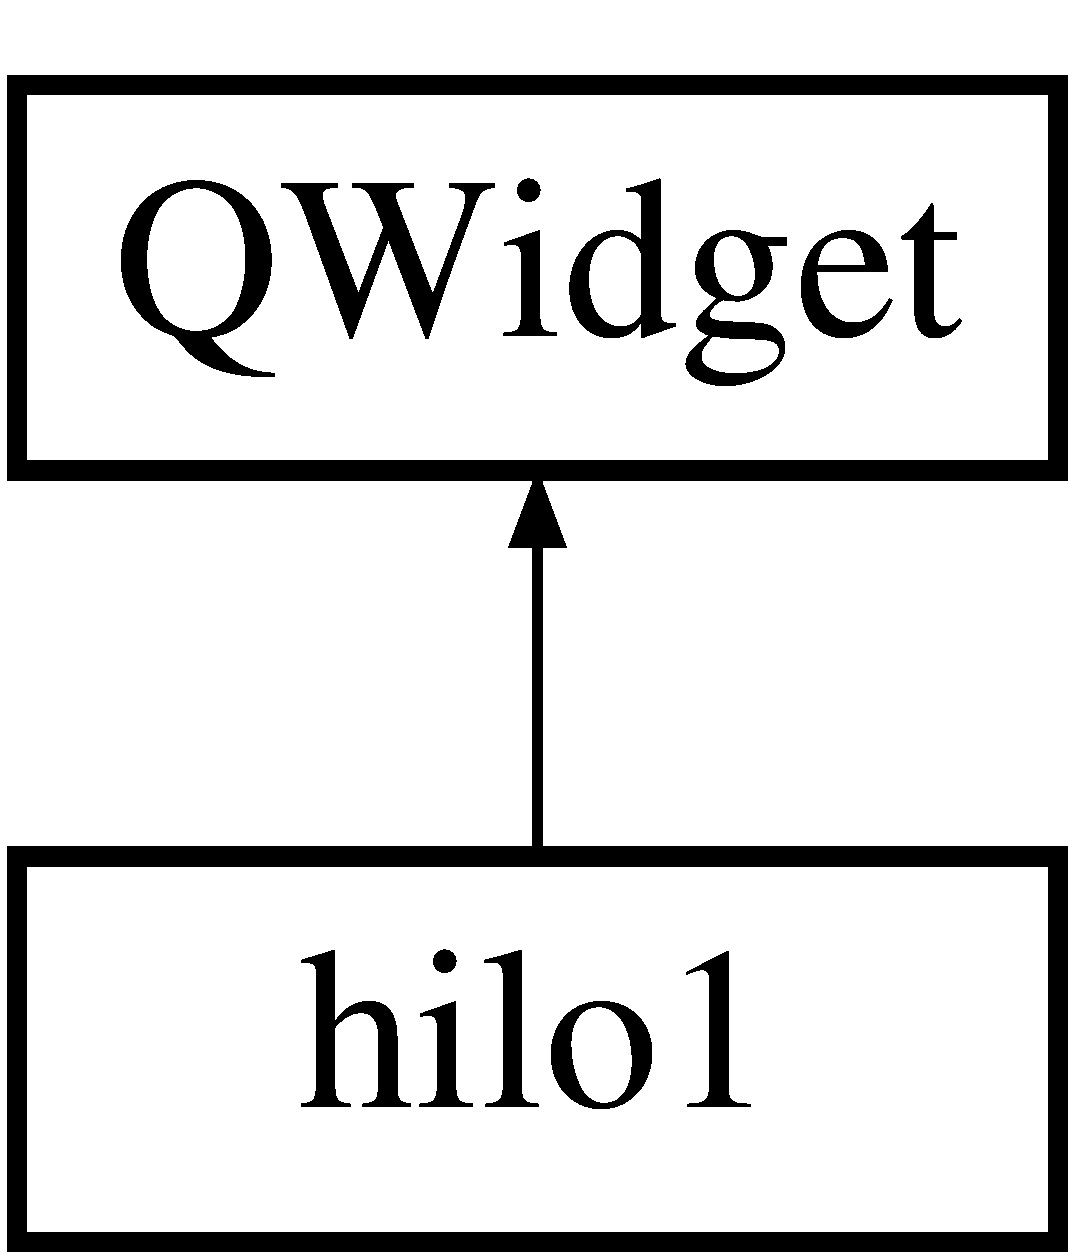
\includegraphics[height=2.000000cm]{classhilo1}
\end{center}
\end{figure}
\subsection*{Métodos públicos}
\begin{DoxyCompactItemize}
\item 
\hypertarget{classhilo1_ac2244f531dad2c953da6cc53f8ad65fa}{{\bfseries hilo1} (Q\-Widget $\ast$parent=0)}\label{classhilo1_ac2244f531dad2c953da6cc53f8ad65fa}

\end{DoxyCompactItemize}
\subsection*{Atributos públicos}
\begin{DoxyCompactItemize}
\item 
\hypertarget{classhilo1_aa69405bbf74d43ea5c5b75f55298cd51}{int {\bfseries h}}\label{classhilo1_aa69405bbf74d43ea5c5b75f55298cd51}

\item 
\hypertarget{classhilo1_a97041e8d73e10802360dfe3d176957f8}{int {\bfseries m}}\label{classhilo1_a97041e8d73e10802360dfe3d176957f8}

\item 
\hypertarget{classhilo1_ac9ad3cf19fd46cbb9f30dfcb5d676ed5}{int {\bfseries s}}\label{classhilo1_ac9ad3cf19fd46cbb9f30dfcb5d676ed5}

\end{DoxyCompactItemize}


La documentación para esta clase fue generada a partir de los siguientes ficheros\-:\begin{DoxyCompactItemize}
\item 
hilo1.\-h\item 
hilo1.\-cpp\end{DoxyCompactItemize}

\hypertarget{classnivel}{\section{Referencia de la Clase nivel}
\label{classnivel}\index{nivel@{nivel}}
}
Diagrama de herencias de nivel\begin{figure}[H]
\begin{center}
\leavevmode
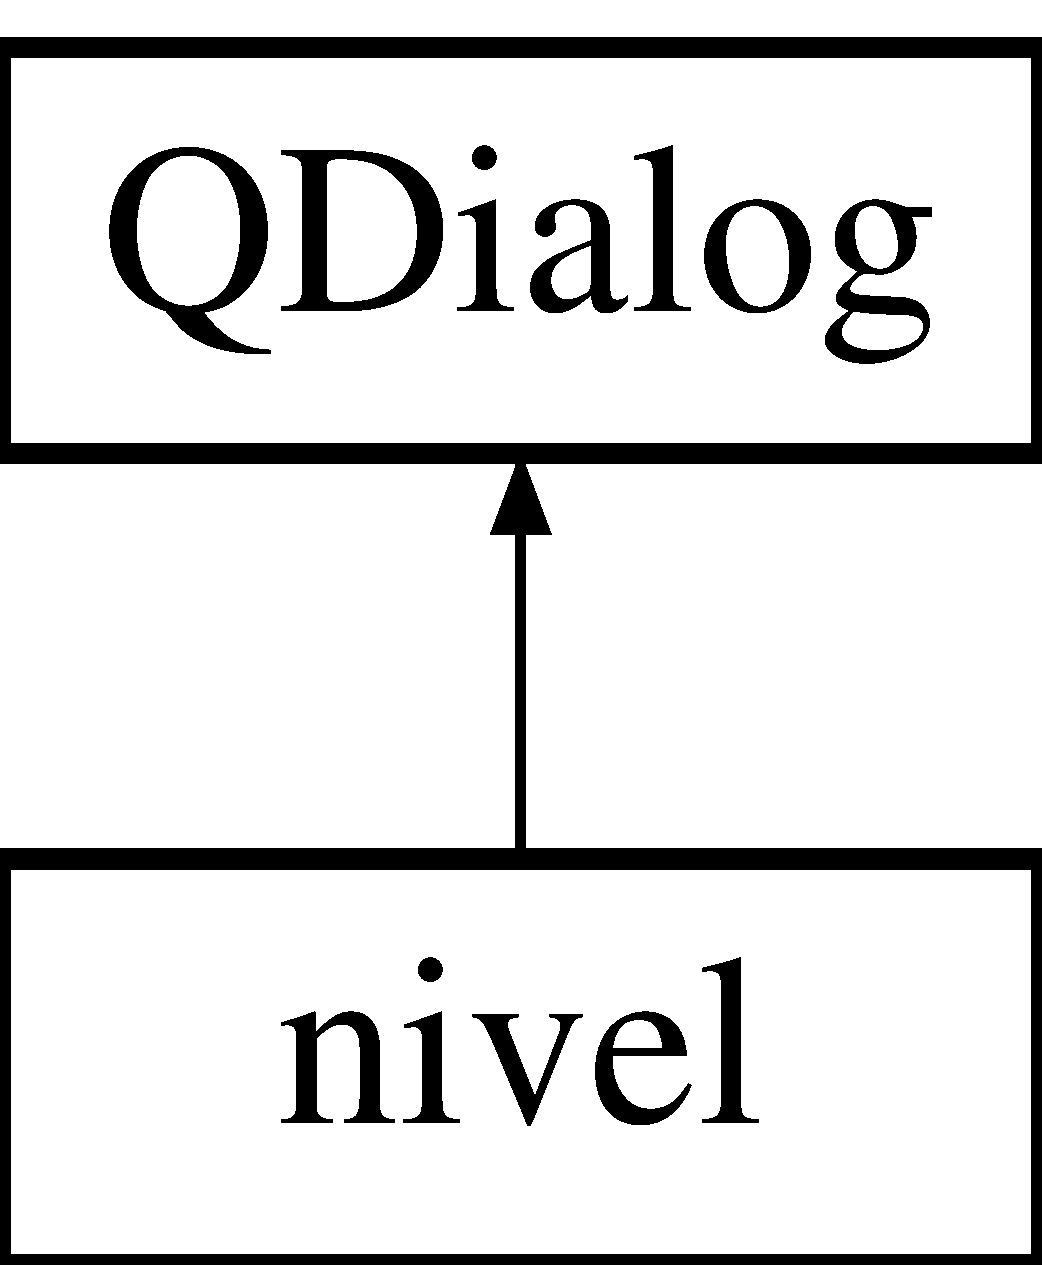
\includegraphics[height=2.000000cm]{classnivel}
\end{center}
\end{figure}
\subsection*{Métodos públicos}
\begin{DoxyCompactItemize}
\item 
\hypertarget{classnivel_add84530f153521109b3c306edf61db1d}{{\bfseries nivel} (Q\-Widget $\ast$parent=0)}\label{classnivel_add84530f153521109b3c306edf61db1d}

\end{DoxyCompactItemize}
\subsection*{Atributos públicos}
\begin{DoxyCompactItemize}
\item 
\hypertarget{classnivel_a63120c4c53d24284ac7fffd1d6382c7b}{int {\bfseries partida}}\label{classnivel_a63120c4c53d24284ac7fffd1d6382c7b}

\item 
\hypertarget{classnivel_aa075fa6ce0af7308326d8debfbbe4217}{Q\-String {\bfseries nom}}\label{classnivel_aa075fa6ce0af7308326d8debfbbe4217}

\item 
\hypertarget{classnivel_a98ab69240e6d5010ee344530c385753f}{\hyperlink{class_q_tablero}{Q\-Tablero} $\ast$ {\bfseries w1}}\label{classnivel_a98ab69240e6d5010ee344530c385753f}

\end{DoxyCompactItemize}


La documentación para esta clase fue generada a partir de los siguientes ficheros\-:\begin{DoxyCompactItemize}
\item 
nivel.\-h\item 
nivel.\-cpp\end{DoxyCompactItemize}

\hypertarget{class_numeros}{\section{Referencia de la Clase Numeros}
\label{class_numeros}\index{Numeros@{Numeros}}
}
Diagrama de herencias de Numeros\begin{figure}[H]
\begin{center}
\leavevmode
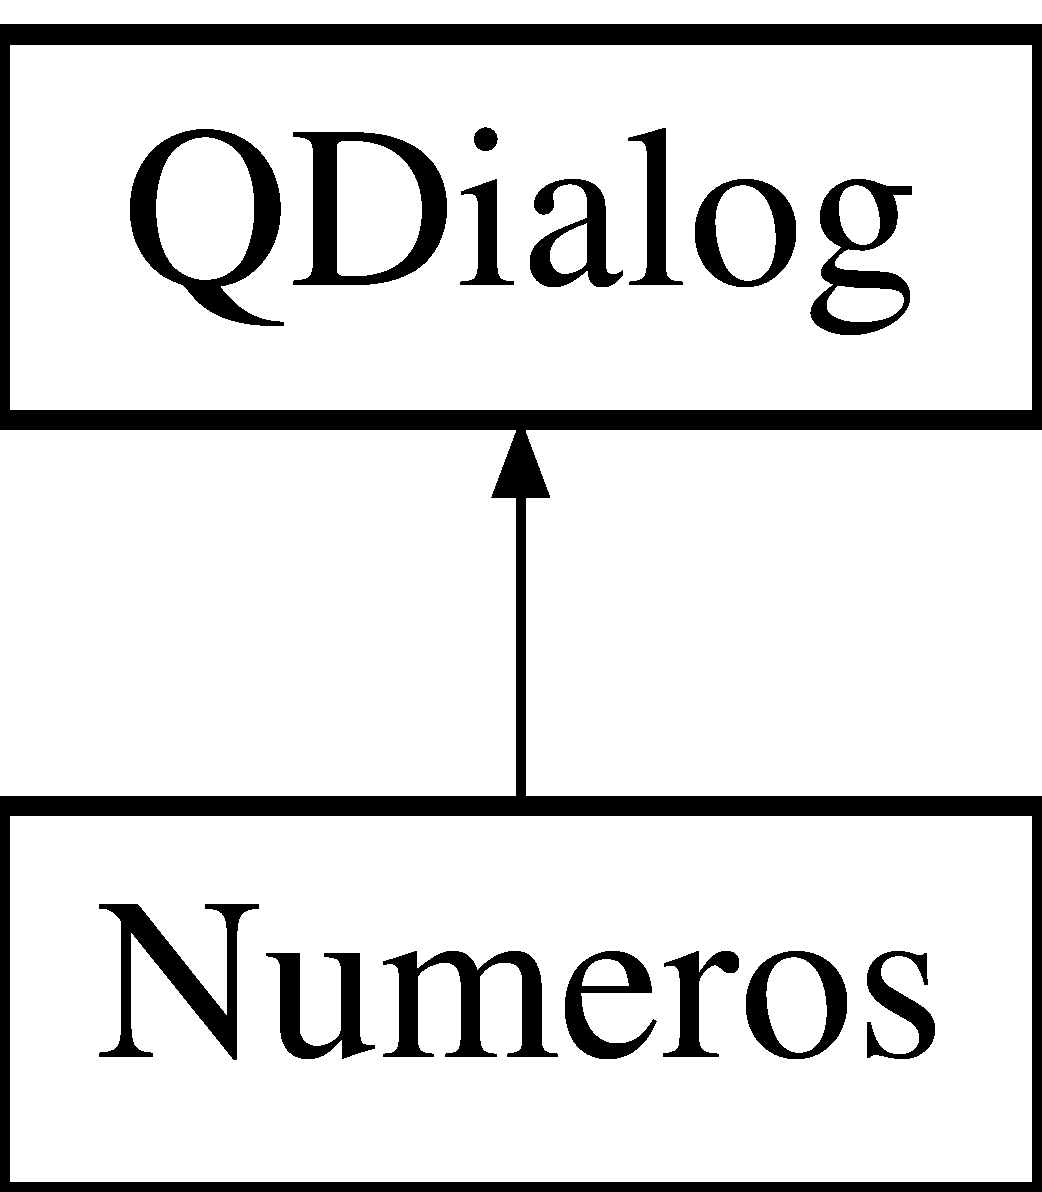
\includegraphics[height=2.000000cm]{class_numeros}
\end{center}
\end{figure}
\subsection*{Métodos públicos}
\begin{DoxyCompactItemize}
\item 
\hypertarget{class_numeros_a6b275591800c3405ed7552b0b03a9077}{{\bfseries Numeros} (Q\-Widget $\ast$parent=0)}\label{class_numeros_a6b275591800c3405ed7552b0b03a9077}

\end{DoxyCompactItemize}
\subsection*{Atributos públicos}
\begin{DoxyCompactItemize}
\item 
\hypertarget{class_numeros_a36867690204e7b9b52bc80249ca5c0bf}{Q\-String {\bfseries numero1}}\label{class_numeros_a36867690204e7b9b52bc80249ca5c0bf}

\end{DoxyCompactItemize}


La documentación para esta clase fue generada a partir de los siguientes ficheros\-:\begin{DoxyCompactItemize}
\item 
numeros.\-h\item 
numeros.\-cpp\end{DoxyCompactItemize}

\hypertarget{classprincipal}{\section{Referencia de la Clase principal}
\label{classprincipal}\index{principal@{principal}}
}
Diagrama de herencias de principal\begin{figure}[H]
\begin{center}
\leavevmode
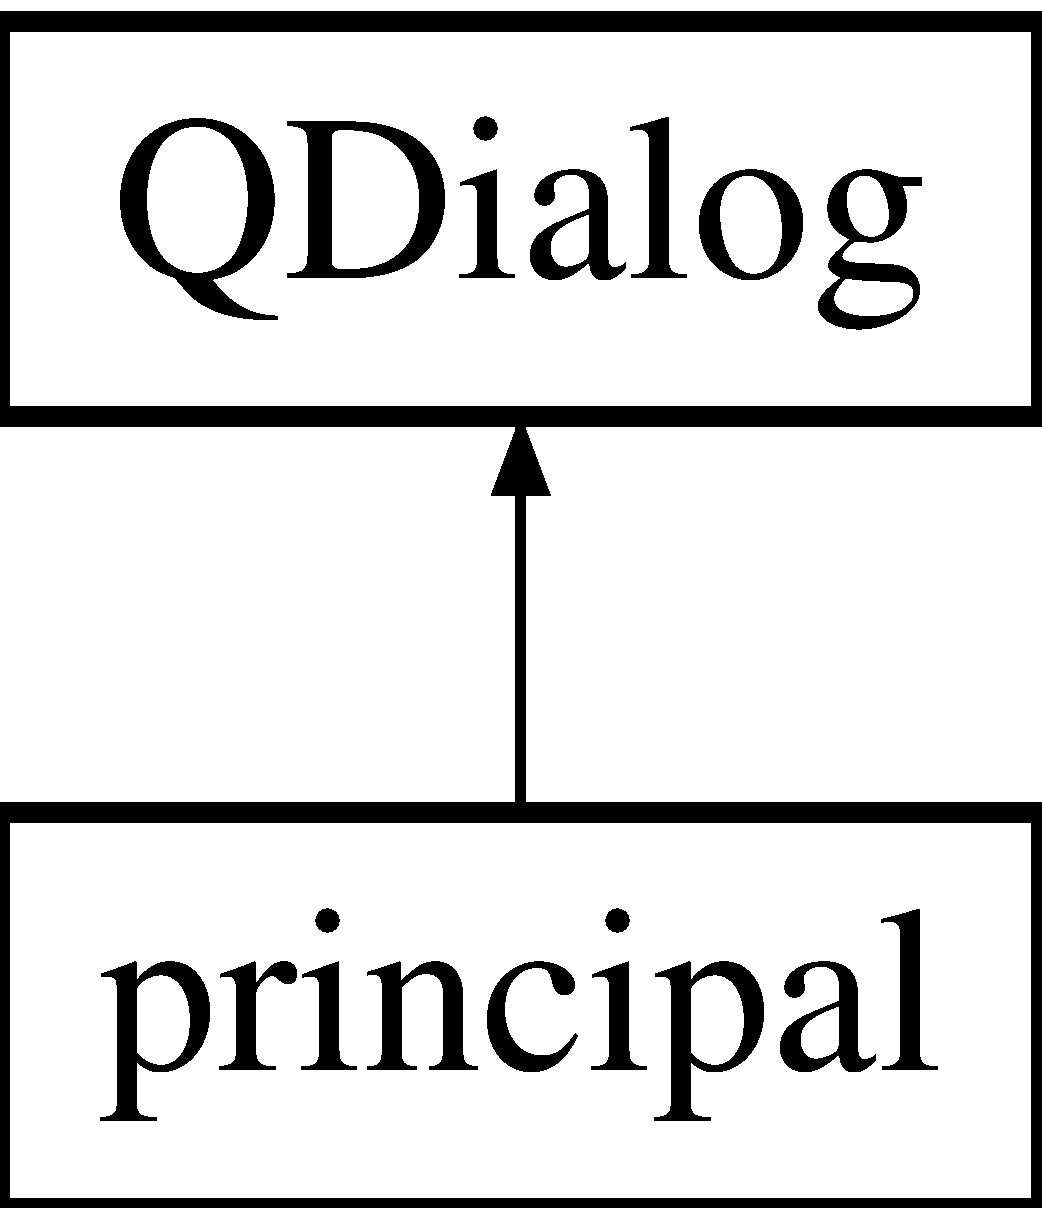
\includegraphics[height=2.000000cm]{classprincipal}
\end{center}
\end{figure}
\subsection*{Métodos públicos}
\begin{DoxyCompactItemize}
\item 
\hypertarget{classprincipal_ab8fd3ebc6c6e93eae9d1ae4ae013cbef}{{\bfseries principal} (Q\-Widget $\ast$parent=0)}\label{classprincipal_ab8fd3ebc6c6e93eae9d1ae4ae013cbef}

\end{DoxyCompactItemize}
\subsection*{Atributos públicos}
\begin{DoxyCompactItemize}
\item 
\hypertarget{classprincipal_a23d9843a5cd1fdd39bfa2aed8f2823ab}{\hyperlink{classnivel}{nivel} $\ast$ {\bfseries w}}\label{classprincipal_a23d9843a5cd1fdd39bfa2aed8f2823ab}

\end{DoxyCompactItemize}


La documentación para esta clase fue generada a partir de los siguientes ficheros\-:\begin{DoxyCompactItemize}
\item 
principal.\-h\item 
principal.\-cpp\end{DoxyCompactItemize}

\hypertarget{class_q_tablero}{\section{Referencia de la Clase Q\-Tablero}
\label{class_q_tablero}\index{Q\-Tablero@{Q\-Tablero}}
}
Diagrama de herencias de Q\-Tablero\begin{figure}[H]
\begin{center}
\leavevmode
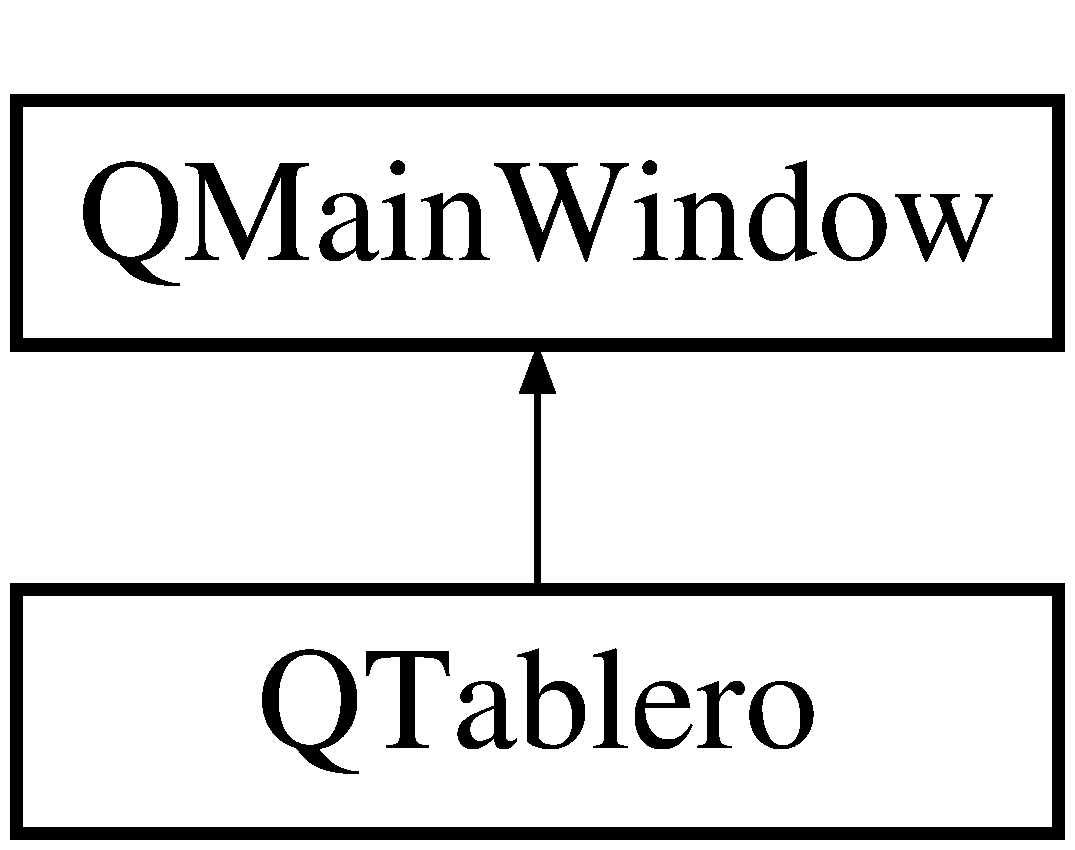
\includegraphics[height=2.000000cm]{class_q_tablero}
\end{center}
\end{figure}
\subsection*{Métodos públicos}
\begin{DoxyCompactItemize}
\item 
\hypertarget{class_q_tablero_ad874f712d2619e753ec1d2e454545d6b}{{\bfseries Q\-Tablero} (Q\-String nombre, Q\-Widget $\ast$parent, int d)}\label{class_q_tablero_ad874f712d2619e753ec1d2e454545d6b}

\end{DoxyCompactItemize}
\subsection*{Atributos públicos}
\begin{DoxyCompactItemize}
\item 
\hypertarget{class_q_tablero_ab6988e6aa07336dc639688ef420f0b10}{Q\-String {\bfseries nombrejugador}}\label{class_q_tablero_ab6988e6aa07336dc639688ef420f0b10}

\item 
\hypertarget{class_q_tablero_a0bd584d1e208a5212d402b30740d4cea}{int {\bfseries dificultad}}\label{class_q_tablero_a0bd584d1e208a5212d402b30740d4cea}

\end{DoxyCompactItemize}


La documentación para esta clase fue generada a partir de los siguientes ficheros\-:\begin{DoxyCompactItemize}
\item 
\hyperlink{qtablero_8h}{qtablero.\-h}\item 
qtablero.\-cpp\end{DoxyCompactItemize}

\chapter{Documentación de archivos}
\hypertarget{qtablero_8h}{\section{Referencia del Archivo qtablero.\-h}
\label{qtablero_8h}\index{qtablero.\-h@{qtablero.\-h}}
}


Este archivo contiene la definicion de la clase Qtablero que nos servira para poder crear el juego Sudoku version 2.\-0.  


{\ttfamily \#include $<$Q\-Main\-Window$>$}\\*
{\ttfamily \#include $<$Q\-Application$>$}\\*
{\ttfamily \#include $<$Q\-File$>$}\\*
{\ttfamily \#include $<$Q\-Time$>$}\\*
{\ttfamily \#include $<$Q\-Debug$>$}\\*
{\ttfamily \#include $<$Q\-Text\-Stream$>$}\\*
{\ttfamily \#include $<$Q\-String$>$}\\*
{\ttfamily \#include $<$Q\-Push\-Button$>$}\\*
{\ttfamily \#include $<$Q\-Grid\-Layout$>$}\\*
{\ttfamily \#include $<$Q\-Text\-Line$>$}\\*
{\ttfamily \#include $<$Q\-Label$>$}\\*
{\ttfamily \#include $<$Q\-Error\-Message$>$}\\*
{\ttfamily \#include $<$Q\-Line\-Edit$>$}\\*
{\ttfamily \#include \char`\"{}numeros.\-h\char`\"{}}\\*
{\ttfamily \#include \char`\"{}hilo1.\-h\char`\"{}}\\*
\subsection*{Clases}
\begin{DoxyCompactItemize}
\item 
class \hyperlink{class_q_tablero}{Q\-Tablero}
\end{DoxyCompactItemize}


\subsection{Descripción detallada}
Este archivo contiene la definicion de la clase Qtablero que nos servira para poder crear el juego Sudoku version 2.\-0. \begin{DoxyAuthor}{Autor}
Marlon Loayza 

Adrian Aguilar
\end{DoxyAuthor}
\begin{DoxyDate}{Fecha}
08/07/2013 
\end{DoxyDate}

%--- End generated contents ---

% Index
\newpage
\phantomsection
\addcontentsline{toc}{part}{Índice}
\printindex

\end{document}
